\documentclass[conference]{IEEEtran}
\synctex=1

%=================================================================
% 
\newcount\DraftStatus  % 0 suppresses notes to selves in text
\DraftStatus=1   % TODO: set to 0 for final version
%=================================================================
\usepackage{comment}
%=================================================================
%
\includecomment{JournalOnly}  
\includecomment{ConferenceOnly}  
\excludecomment{TulipStyle}
%
%=================================================================
%=================================================================
% gitlatexdiff
%
%  https://gitlab.com/git-latexdiff/git-latexdiff
%=================================================================
%  git latexdiff HEAD  HEAD~5 --main templatex.tex
%  git latexdiff HEAD~1  --main templatex.tex
%  View pdf to see difference
%
%=================================================================
%
% Todo Notes for marginal comments
% 
%\newcount\DraftStatus  % 0 suppresses notes to selves in text
%\DraftStatus=1   % TODO: set to 0 for final version
\ifnum\DraftStatus=1
	\usepackage[draft,colorinlistoftodos,color=orange!30]{todonotes}
\else
	\usepackage[disable,colorinlistoftodos,color=blue!30]{todonotes}
\fi 
%\usepackage[disable]{todonotes} % notes not showed
%\usepackage[draft]{todonotes}   % notes showed
%
\makeatletter
 \providecommand\@dotsep{5}
 \def\listtodoname{List of Todos}
 \def\listoftodos{\@starttoc{tdo}\listtodoname}
 \makeatother
%
%=================================================================
%
\usepackage{color}
\newcommand{\draftnote}[3]{ 
	\todo[author=#2,color=#1!30,size=\footnotesize]{\textsf{#3}}	}
% TODO: add yourself here:
%
\newcommand{\gangli}[1]{\draftnote{blue}{GLi:}{#1}}
\newcommand{\qwu}[1]{\draftnote{red}{QWu:}{#1}}
\newcommand{\gliMarker}
	{\todo[author=GLi,size=\tiny,inline,color=blue!40]
	{Gang Li has worked up to here.}}
\newcommand{\qwuMarker}
	{\todo[author=QWu,size=\tiny,inline,color=red!40]
	{Qiong Wu has worked up to here.}}
%=================================================================

%=================================================================
%
% general packages
%  https://en.wikibooks.org/wiki/Category:Book:LaTeX
%  https://en.wikibooks.org/wiki/LaTeX/Package_Reference
%
%=================================================================
\usepackage{graphicx}
\usepackage{algorithm}
\usepackage{algorithmic}
\usepackage{breqn}
\usepackage{subfigure}
\usepackage{multirow}
\usepackage{psfrag}
\usepackage{url}
\usepackage[colorlinks]{hyperref}
\usepackage{booktabs}
\usepackage{rotating}
\usepackage{colortbl}
\usepackage{paralist}
%\usepackage{geometry}
\usepackage{epstopdf}
\usepackage{nag}
\usepackage{microtype}
\usepackage{siunitx}
\usepackage{nicefrac}
% for random text
\usepackage{lipsum}
\usepackage[english]{babel}
\usepackage[pangram]{blindtext}
%
%=================================================================


%=================================================================
%
% Version control information
%
%=================================================================
\usepackage{gitinfo2}
%=================================================================
\begin{NonSpringer}
\usepackage{natbib}
\usepackage{fancyhdr}
\pagestyle{fancy}
\fancyhead{} % clear all header fields
\fancyhead[RO,LE]{\textsl{\rightmark}}
\fancyhead[LO,RE]{\ensuremath{\Rightarrow}
		\textbf{\textbf{[CONFIDENTIAL]}}\ensuremath{\Leftarrow}}
\fancyhead[CO,CE]{}
%=================================================================
\fancyfoot{} % clear all footer fields
\fancyfoot[CE,CO]{\textbf{\thepage}} 
\fancyfoot[LO,LE]{
\includegraphics[height=.9\headheight]{figures/tulip-icon.png}
		\gitVtagn-\gitBranch\ (\gitCommitterDate)}
\fancyfoot[RO,RE]{Committed by: \textsl{\gitCommitterName}}

\setlength{\headheight}{12pt}
\renewcommand{\headrulewidth}{0.4pt}
\renewcommand{\footrulewidth}{0.4pt}
%=================================================================

%=================================================================
% for math notations
% ----------------------------------------------------------------
\usepackage{mathtools}
\usepackage{amsthm}
%
% THEOREMS -------------------------------------------------------
%
\newtheorem{thm}{Theorem}[section]
\newtheorem{cor}[thm]{Corollary}
\newtheorem{lem}[thm]{Lemma}
\newtheorem{prop}[thm]{Proposition}
\theoremstyle{definition}
\newtheorem{defn}[thm]{Definition}
\theoremstyle{remark}
\newtheorem{rem}[thm]{Remark}
\numberwithin{equation}{section}
% MATH -----------------------------------------------------------
\newcommand{\norm}[1]{\left\Vert#1\right\Vert}
\newcommand{\abs}[1]{\left\vert#1\right\vert}
\newcommand{\set}[1]{\left\{#1\right\}}
\newcommand{\Real}{\mathbb R}
\newcommand{\eps}{\varepsilon}
\newcommand{\To}{\longrightarrow}
\newcommand{\BX}{\mathbf{B}(X)}
% ----------------------------------------------------------------
\newcommand{\I}{{\cal I}}
\newcommand{\Id}{{\cal I} }
\newcommand{\Dc}{{\cal D}}
\newcommand{\J}{{\cal J}}
\newcommand{\Dn}{{\cal D}_n}
\newcommand{\Dd}{{\cal D}_n }
\renewcommand{\P}{{\cal P}}
\newcommand{\Nu}{{\cal N} }
\newcommand{\B}{{\cal B}}
\newcommand{\Bf}{{\bf B}}
\newcommand{\Y}{{\bf Y}}
\newcommand{\A}{{\cal A}}
% ----------------------------------------------------------------
\newcommand{\V}{{\cal V}}
\newcommand{\M}{{\cal M}}
\newcommand{\F}{{\cal F}}
\newcommand{\Fd}{{\cal F}}
\newcommand{\BF}{{\cal BF}_n}
\newcommand{\BFd}{{\cal BF}_n}
\newcommand{\TF}{{\cal TF}_n}
\newcommand{\TFd}{{\cal TF}_n}
\newcommand{\G}{{\cal G}}
\newcommand{\X}{{\cal X}}
\newcommand{\E}{{\cal E}}
\newcommand{\K}{{\cal K}}
\newcommand{\T}{{\cal T}_n}
\renewcommand{\H}{{\cal H}}
% ----------------------------------------------------------------
\newtheorem{Remark}{Remark}
\newtheorem{proposition}{Proposition}
\newtheorem{theorem}{Theorem}
\newtheorem{lemma}{Lemma}
\newtheorem{corollary}{Corollary}
\newtheorem{example}{Example}
\newtheorem{definition}{Definition}
\newtheorem{Algorithms}{Algorithm}
% ----------------------------------------------------------------
\newcommand{\bu}{{\mathbf 1} }
\newcommand{\bo}{{\mathbf 0} }
\newcommand{\N}{\mbox{{\sl l}}\!\mbox{{\sl N}}}
% ----------------------------------------------------------------
\def\uint{[0,1]}
\def\proof{{\scshape Proof}. \ignorespaces}
\def\endproof{{\hfill \vbox{\hrule\hbox{%
   \vrule height1.3ex\hskip1.0ex\vrule}\hrule
  }}\par}
%
%=================================================================
\end{NonSpringer}

\usepackage{cleveref}



\hypersetup
{
    pdfauthor={\gitAuthorName},
    pdfsubject={TULIP Lab},
    pdftitle={},
    pdfkeywords={TULIP Lab, Data Science},
%	bookmarks=true,  
}






\def\BibTeX{{\rm B\kern-.05em{\sc i\kern-.025em b}\kern-.08em
    T\kern-.1667em\lower.7ex\hbox{E}\kern-.125emX}}

%=================================================================
%
\begin{document}
%
%=================================================================
% Preamble which will need to be changed for submission
%
\title{Title of This Paper*
\thanks{Thanks for the funding XXX-XXXXX.}
}

\author{\IEEEauthorblockN{X. YY}
\IEEEauthorblockA{\textit{School of Information Technology} \\
\textit{Deakin University, Geelong, Australia}\\
gang.li@deakin.edu.au}
\and
\IEEEauthorblockN{Gang Li}
\IEEEauthorblockA{\textit{School of Information Technology} \\
\textit{Deakin University, Geelong, Australia}\\
gang.li@deakin.edu.au}
\and
\IEEEauthorblockN{3\textsuperscript{rd} Given Name Surname}
\IEEEauthorblockA{\textit{dept. name of organization (of Aff.)} \\
\textit{name of organization (of Aff.)}\\
City, Country \\
email address}
}

\maketitle

\begin{abstract}
The abstract will be put here, ....
\end{abstract}

\begin{IEEEkeywords}
component, formatting, style, styling, insert
\end{IEEEkeywords}


%=================================================================

%=================================================================
\section{Introduction}
\label{sec-intro}

Deep learning has been studied in many research fields, such as image recognition, natural language processing and prediction system. In short, deep learning is a new field in machine learning. Its motivation is to build and simulate the neural network of human brain for analytical learning. It imitates the mechanism of human brain to interpret data.\\

In this study, we take out several key factors that affect the final business income, such as early investment, popularity, time and so on, and build a two-layer neural network to predict the film revenue. Then these key values are put into the neural network as feature input, and then the back propagation of BF neural network is used to update the weights, and finally the prediction model is obtained.\\
   
This paper aims at the existing methods to solve the practical problems of the film industry, so that the film industry can use the effective data to predict the possible revenue of making a film. The experimental results show that using neural network to solve the film revenue is a very desirable method.\\























\section{Related Work} \label{sec-preliminaries}

First of all, our work can be divided into the following steps:   \\
(1) Data download: the data source is directly downloaded and used from the kaggle project.\\
\begin{center}
  \begin{minipage}{0.3\linewidth}
  \centering

  \includegraphics[width=0.9\textwidth]{logos/21.eps}
 
  {\small{Flag.1}}

  \end{minipage}
  \hfill
\end{center}
(2) Data cleaning: delete some unimportant or less influential data, such as poster_ path,overview,imdb_ ID, homepage, etc \\
\begin{center}
  \begin{minipage}{0.3\linewidth}
  \centering

  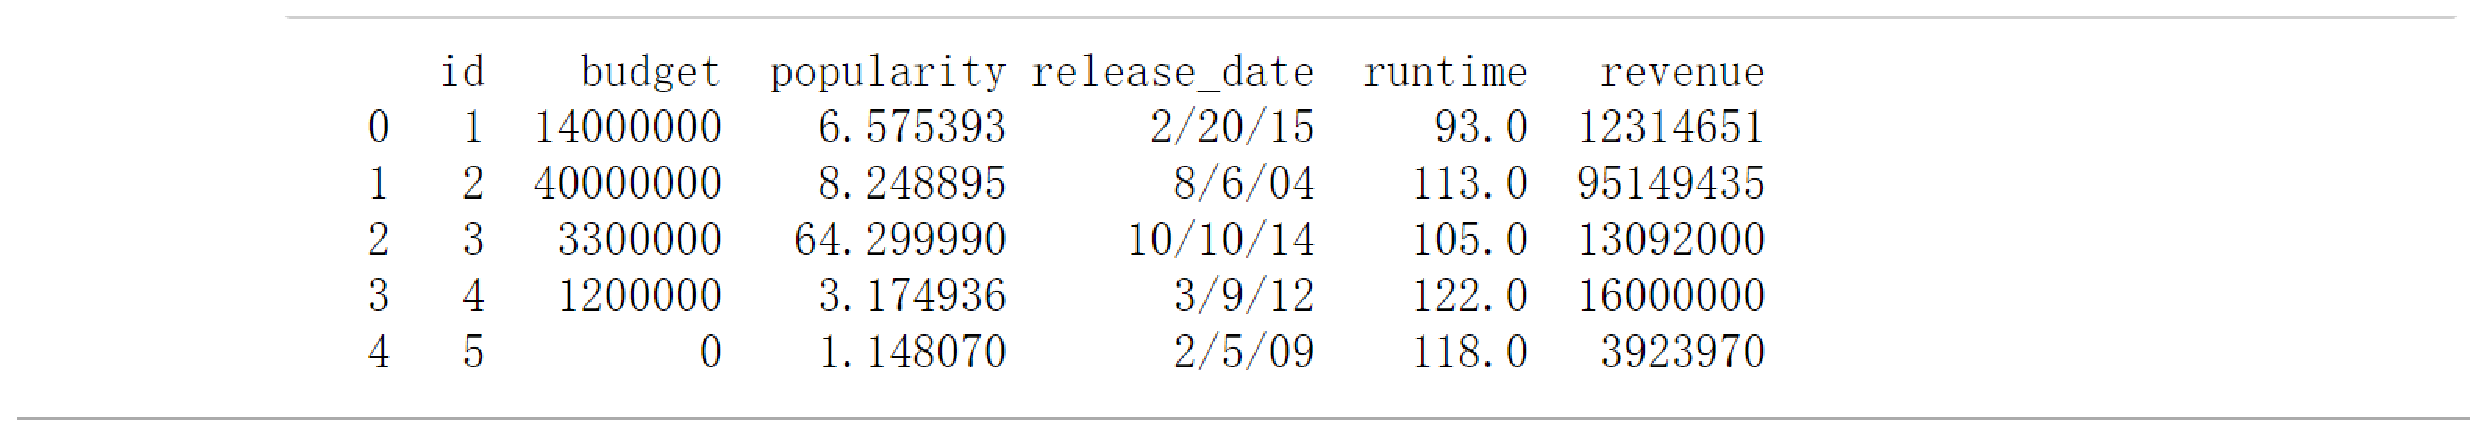
\includegraphics[width=0.9\textwidth]{logos/24.eps}
 
  {\small{Flag.1}}

  \end{minipage}
  \hfill
\end{center}
(3) Data analysis: To observe the impact of previous investment on the film, we use Matplotlib in Python to draw a picture, flag 1, we can see that the investment is directly proportional to the business income.

\begin{center}
  \begin{minipage}{0.3\linewidth}
  \centering

  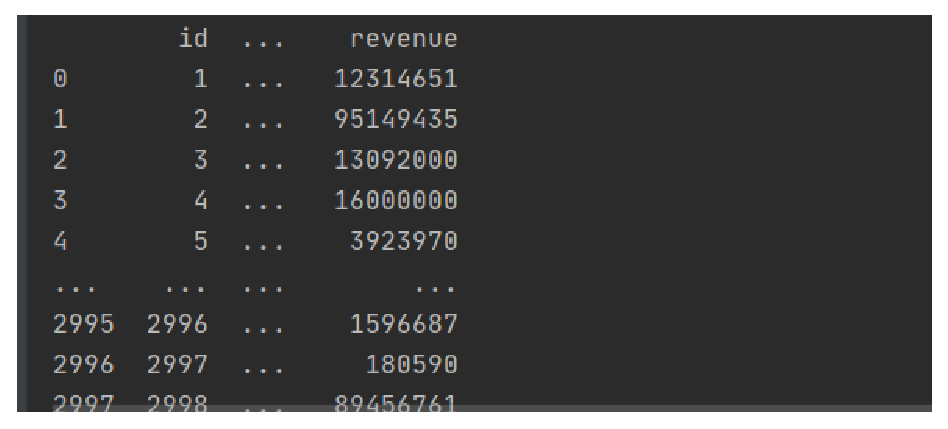
\includegraphics[width=0.9\textwidth]{logos/4.eps}
 
  {\small{Flag.1}}

  \end{minipage}
  \hfill
\end{center}

To observe the impact of previous investment on the film, we use Matplotlib in Python to draw a picture, flag 1, we can see that the investment is directly proportional to the business income.

\begin{center}
  \begin{minipage}{0.3\linewidth}
  \centering

  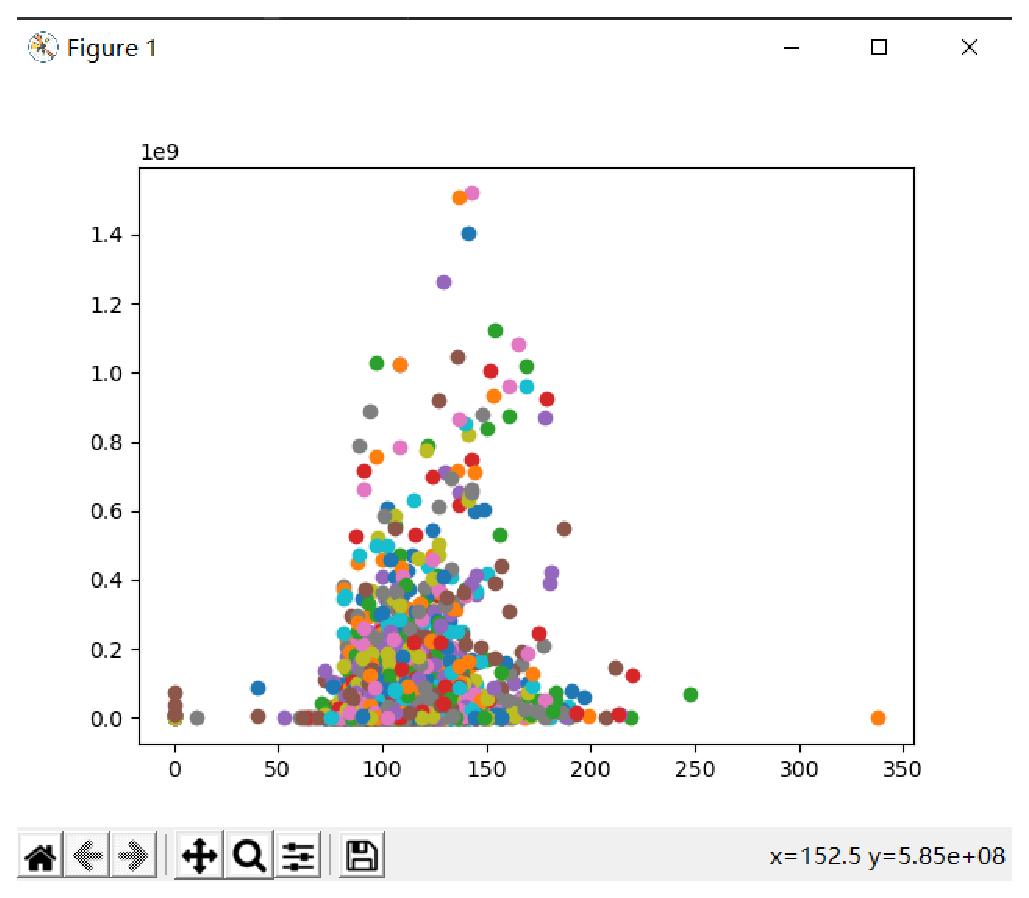
\includegraphics[width=0.9\textwidth]{logos/22.eps}
 
  {\small{Flag.1}}

  \end{minipage}
  \hfill
\end{center}
To observe the impact of previous investment on the film, we use Matplotlib in Python to draw a picture, flag 1, we can see that the investment is directly proportional to the business income.

\begin{center}
  \begin{minipage}{0.3\linewidth}
  \centering

  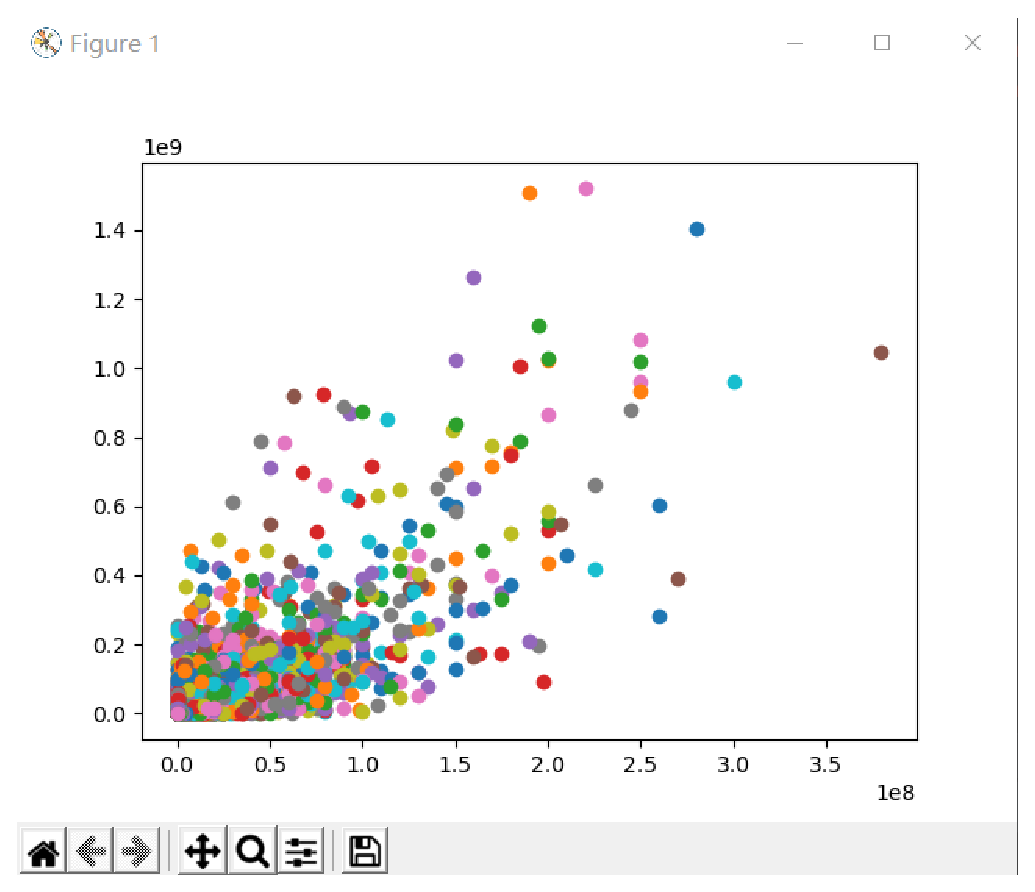
\includegraphics[width=0.9\textwidth]{logos/25.eps}
 
  {\small{Flag.1}}

  \end{minipage}
  \hfill
\end{center}
To observe the impact of previous investment on the film, we use Matplotlib in Python to draw a picture, flag 1, we can see that the investment is directly proportional to the business income.

\begin{center}

  \begin{minipage}{0.3\linewidth}
  \centering

  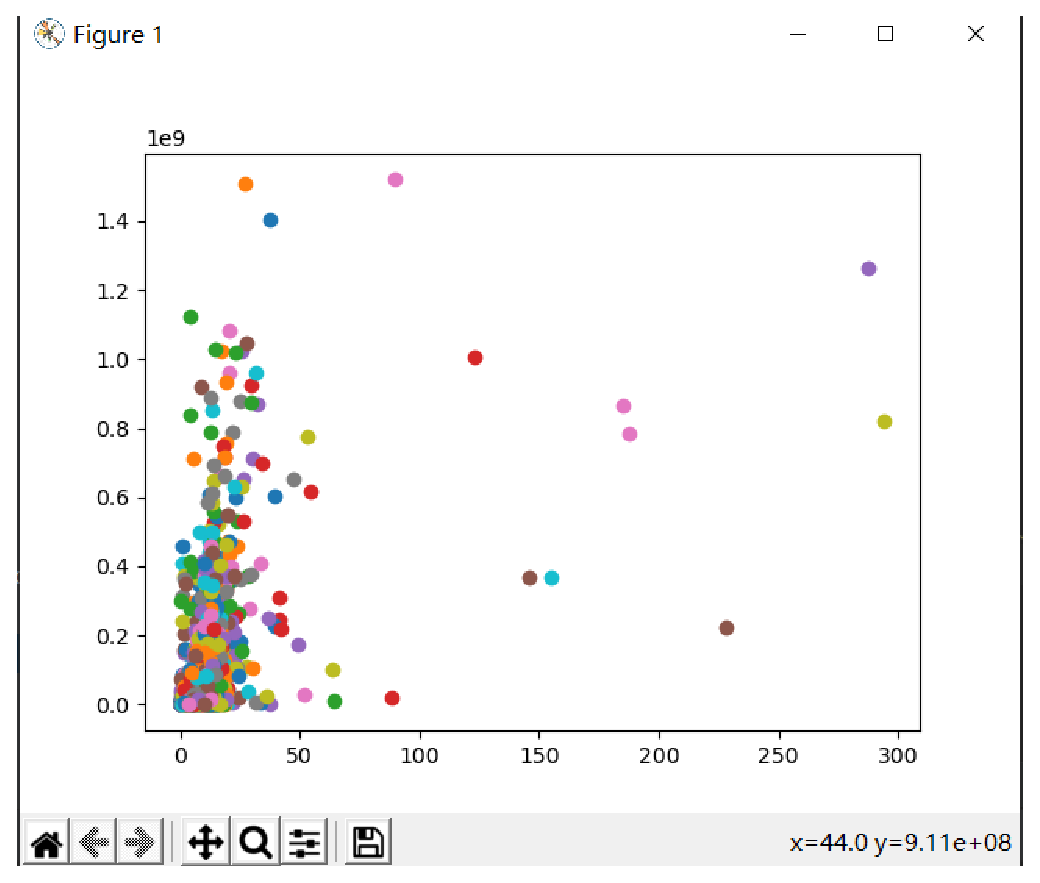
\includegraphics[width=0.9\textwidth]{logos/26.eps}
  
  {\small{The relationship between popularity and business income}}

  \end{minipage}
\end{center}
}


\section{Methodology} 


In this section, we will introduce our methodology framework. We use a three-layer neural network. There are 64 neurons in the first layer, 64 neurons in the second layer, and 1 neuron in the last layer,            Finally, the cost function is selected as the square difference, and the design figure flag. 5
\begin{center}

  \begin{minipage}{0.3\linewidth}
  \centering

  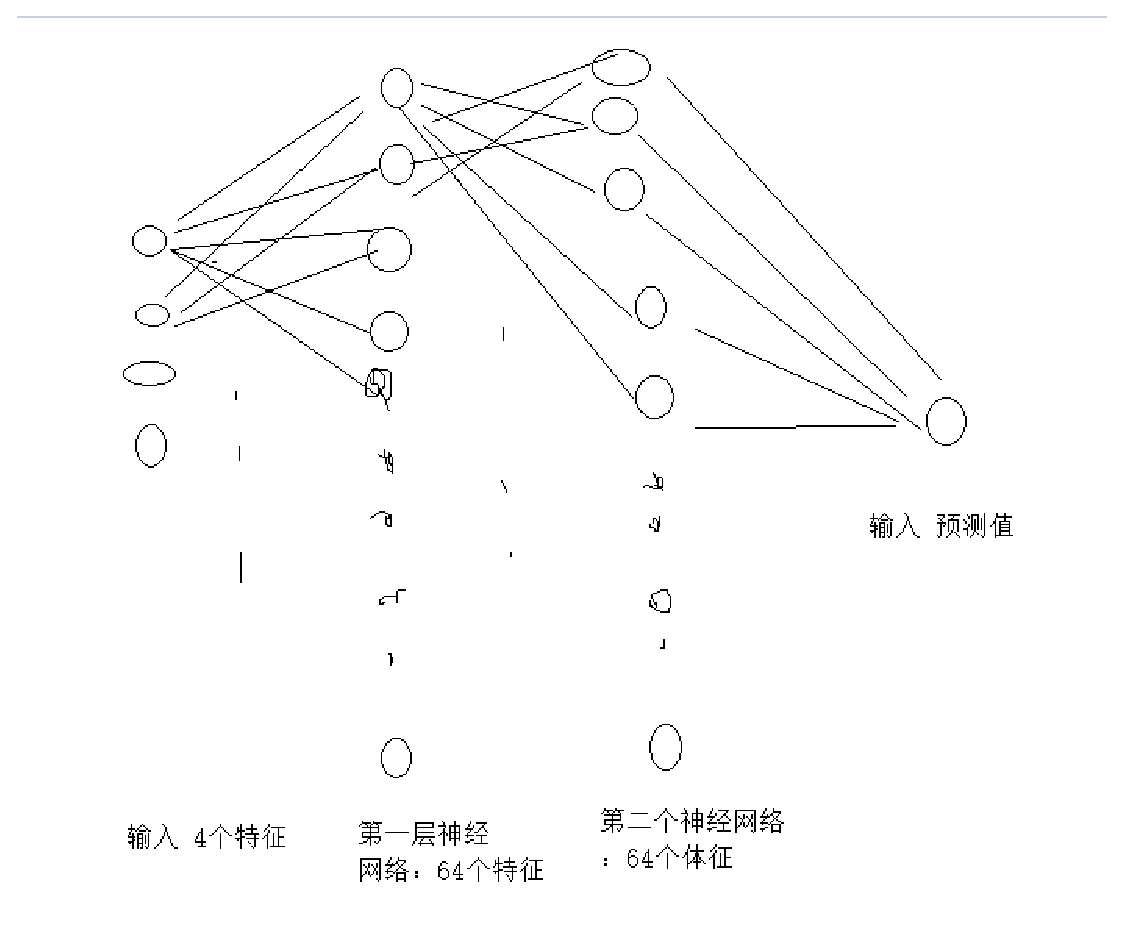
\includegraphics[width=0.9\textwidth]{logos/7.eps}
  
  {\small{The relationship between popularity and business income}}

  \end{minipage}
\end{center}


3.1 parameter learning \\
From the data analysis, we select several parameters which have the greatest impact on the business income as X. the weights of the first layer of neural network are W1 and bias value B1, the weight of the second layer of neural network is W2 and bias value B1, and the third layer of neural network W3 and bias value B1.\\ 
The first layer of neural network is: Z1 = relu (w1x + B1) \\
The second layer neural network is: Z2 = relu (w2z1 + B1) \\
The second layer neural network is: Z3 = relu (w3z2 + B1) \\
We get W1, W2 and W3 by neural network updating

\section{Experiment} \label{sec-experiment}
4.1 Dataset\\
We downloaded data sets from the kaggle project, including test sets (including 3000 data sets) and training sets (1000 data sets). The dataset contains budget, genre, home page, IMDB_ ID, original language, original title, overview, popularity, poster path, production company, production country, release date, running time, spoken language, status, slogan, title, keywords, actors, staff, etc. Delete the weights that are not important or have little impact on the dataset, leaving only the feature values with large weight influence, such as budget, release date, running time, popularity, etc.\\
4.2 Hyper-parameter Settings\\
The training model of this neural network has three layers. The corresponding weights are W1, W2 and W3. The cost function is designed as mean square error, learning rate Le = 0.01, update times 200, each time 200 data.\\
4.3 Overall Performance\\
Firstly, for the overall analysis, we forecast from these aspects:\\
(1) The update rate of cost function is the cost function of mean square error. We can clearly see that after 10 times of updating, the loss value of his cost function remains around 8000.\\
\begin{center}

  \begin{minipage}{0.3\linewidth}
  \centering

  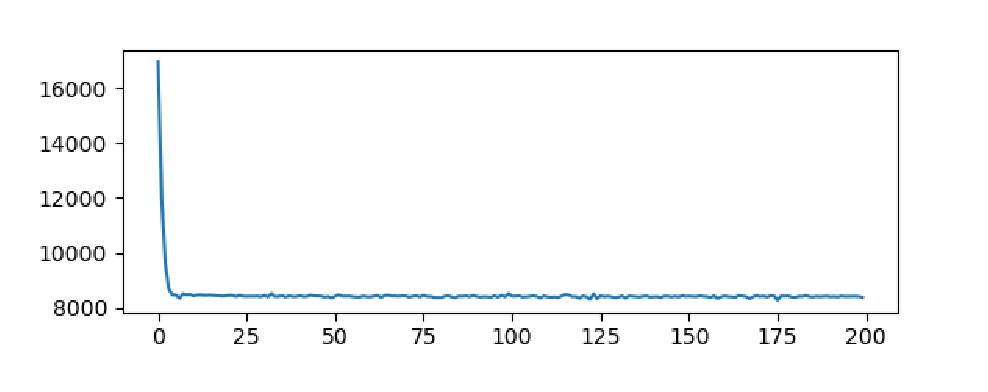
\includegraphics[width=0.9\textwidth]{logos/1 (1).eps}
  
  {\small{cost}}

  \end{minipage}
\end{center}
(2) The difference between the actual value and the predicted value, we can clearly see that the difference between the actual value and the final actual value is about 46.
\begin{center}

  \begin{minipage}{0.3\linewidth}
  \centering

  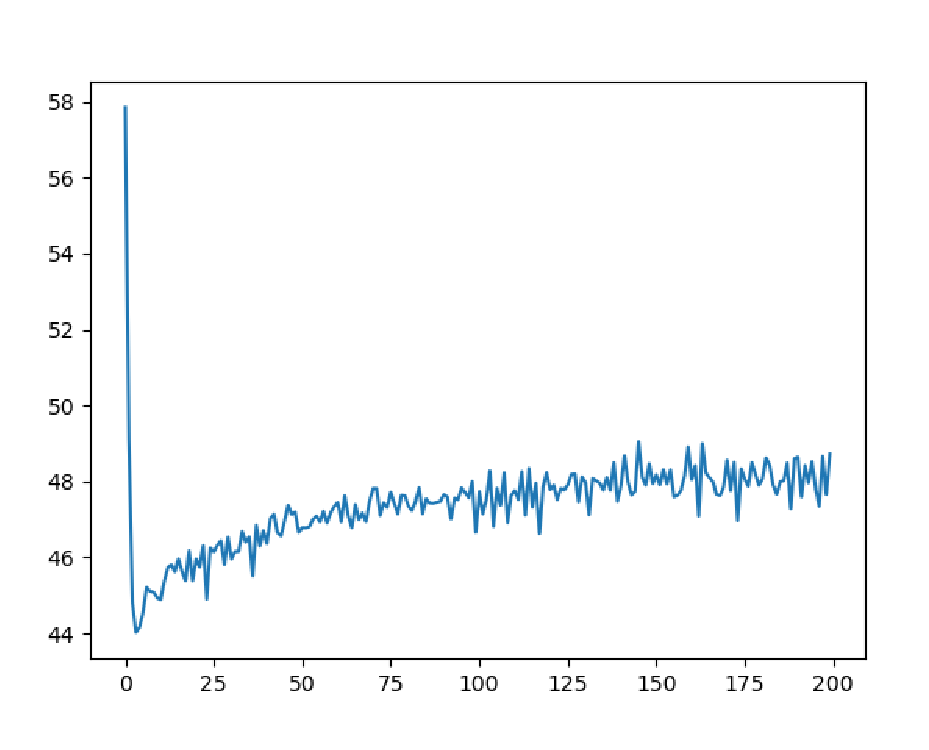
\includegraphics[width=0.9\textwidth]{logos/1 (2).eps}
  
  {\small{cost}}

  \end{minipage}
\end{center}

4.4 Forecast\\
We input the test data into the model and test the model to give the predicted value of movie evaluation.
\begin{center}

  \begin{minipage}{0.3\linewidth}
  \centering

  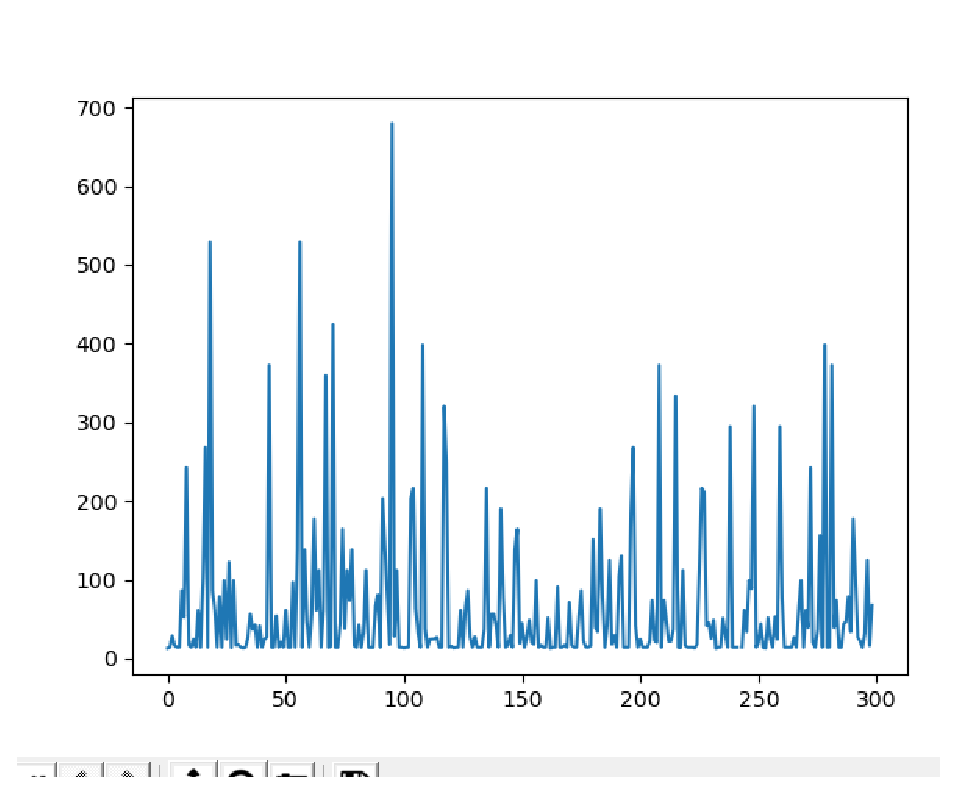
\includegraphics[width=0.9\textwidth]{logos/1 (3).eps}
  
  {\small{cost}}

  \end{minipage}
\end{center}
\section{Conclusions}

This paper combines deep learning with practice and application to solve the prediction value of profit demanded by the film industry. In our experiment, we compare each factor, compare it with the film profit factor, and make corresponding image display. And we use the neural network related knowledge design model structure, training, get a good result, from the final experimental results, the cost function is small to 8000, the square difference between the predicted value and the actual value is about 46, the effect is also good. In the future, we plan to use multi task learning to improve the method and improve the accuracy of prediction.


% ----------------------------------------------------------------
\newpage
%\bibliographystyle{plain}
\bibliographystyle{newapa}
\bibliography{tulipbib}
%=================================================================

\listoftodos

\end{document}

